\chapter{Week 01: Planning}
\section{Motivation for choosing architecture}
%\paragraph{
Motivation for choosing architecture:
For our initial architecture we choose DC-GAN, because our task is to generate new images based on a given dataset. We believe that the structure of having a generator and discriminator would lead to the results we want.
For the training, we would like to begin from WGAN-GP(Wasserstein GAN with gradient penalty) as training method, which gives a significant improvement by stability of training. So far we tested different GAN variants (vanilla GAN, WGAN and WGAN-GP) on the MNIST Dataset. WGAN-GP showed a prominent improvement in the outcome.
% Which the last is using a better loss function for training.


As to VAE, VAE tends to generate imagines that somehow blurry. We test the example code of pyro. So we have not chosen it.
%}


\begin{figure}[H]
    \centering
    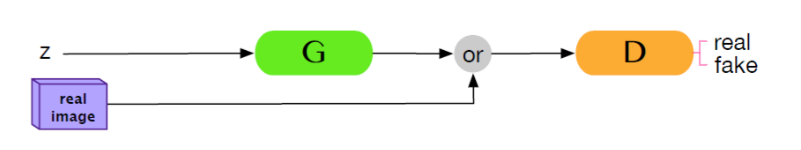
\includegraphics[height=3cm]{images/dc-gan_layout.png}
    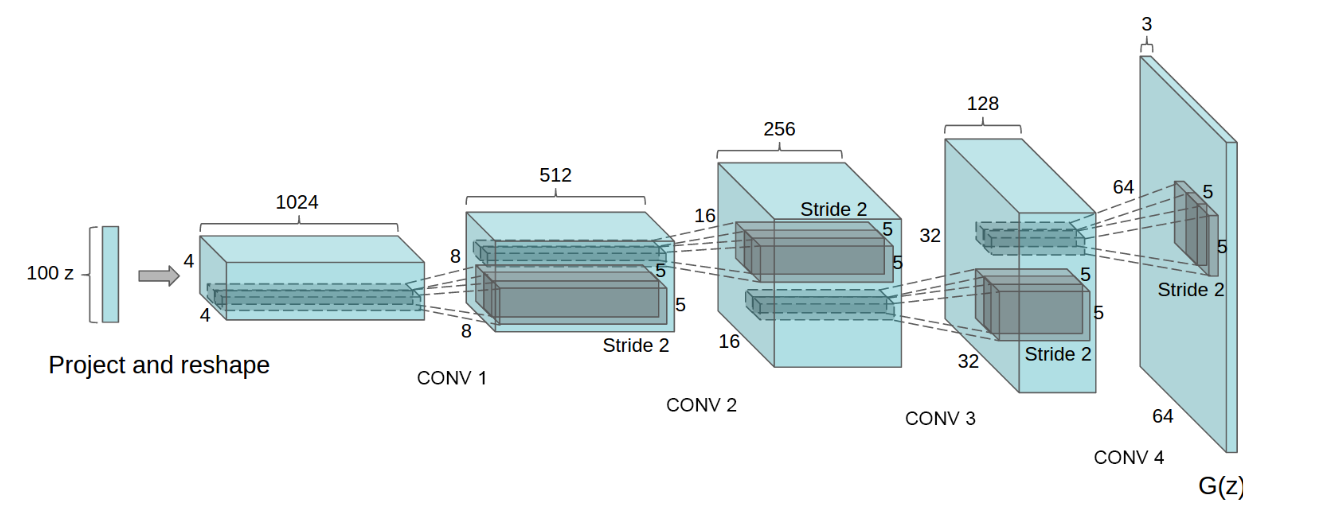
\includegraphics[height=6cm]{images/dc-gan_example.png}
    \caption{Basic architecture as presented in the lecture}
    \label{fig:dc-gan-example}
\end{figure}




\newpage
\chapter{Week 02: Implementation 1}
\section{Work about loading the data}
\paragraph{
As you can see in the code snippet below, we implemented the data loader. In \ref{fig:dataplot}, we plotted 64 randomly picked images. While looking at the metadata, we noticed that for some of the data points, certain attributes were missing. Some images did not have the age of the patient or the analytical method used to find about the type of skin lesion. For those we have to think about how to fill in the missing attributes in the future. Looking into the metadata, we also thought about generating skin lesion images from certain attributes, e.g. a skin lesion image of a patient of a certain age. But because this is not the main focus for now, we postponed that thought and will come back to it later, when we have a working prototype. Lastly, we created a Github repository to maintain our code at one place as we also have written the boilerplate code for the DC-GAN.
}

\begin{figure}[htbp]
    \centering
    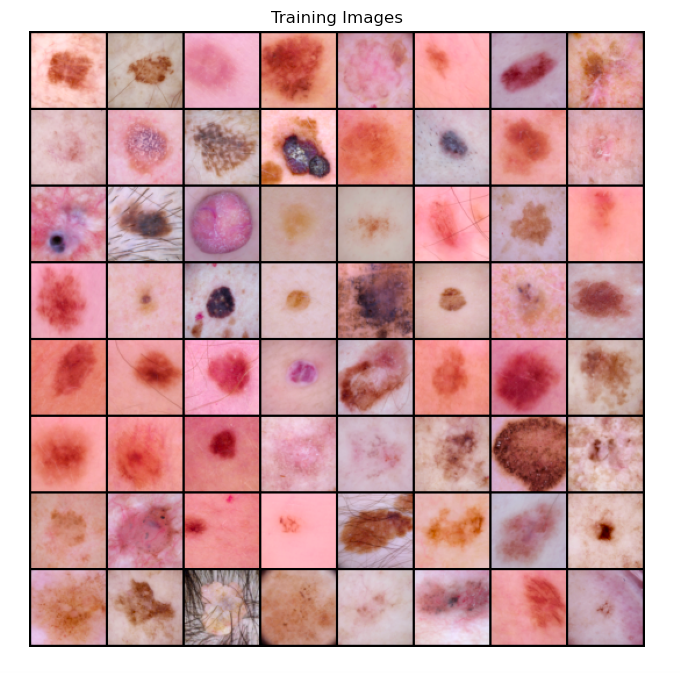
\includegraphics[width=5in]{images/sample_plot.png}
    \label{fig:dataplot}
\end{figure}

\begin{lstlisting}
import copy
import glob
import logging

import torch
import torch.cuda
from PIL import Image
from torch.utils.data import Dataset
from torchvision.transforms import transforms

from dataloader.process_meta_data import get_lesion_infos

log = logging.getLogger(__name__)
# log.setLevel(logging.WARN)
# log.setLevel(logging.INFO)
log.setLevel(logging.DEBUG)


class SkinLesionDataset(Dataset):
    def __init__(self,
                 val_stride=0,
                 is_validation=None,
                 lesion_id=None,
                 transform=None,
                 ):
        if transform:
            self.transform = transform
        else:
            self.transform = transforms.ToTensor()

        self.lesion_infos = copy.copy(get_lesion_infos())

        self.jpgs_paths = glob.glob('/usr/src/rawdata/*.jpg')

        if lesion_id:
            self.lesion_infos = [
                x for x in self.lesion_infos if x.lesion_id == lesion_id
            ]

        if is_validation:
            assert val_stride > 0, val_stride
            self.lesion_infos = self.lesion_infos[::val_stride]
            assert self.lesion_infos
        elif val_stride > 0:
            del self.lesion_infos[::val_stride]
            assert self.lesion_infos

        log.info('{!r}: {} {} samples'.format(
            self,
            len(self.lesion_infos),
            'validation' if is_validation else 'training',
        ))

    def __len__(self):
        return len(self.lesion_infos)

    def __getitem__(self, idx):
        lesion_infos_tup = self.lesion_infos[0][idx]
        image_path = ''
        for path in self.jpgs_paths:
            image_id = path.split('/')[-1].split('.')[0]
            if image_id == lesion_infos_tup.image_id:
                image_path = path
                break

        if len(image_path) == 0:
            log.error('{!r}: {} was not found in dataset'.format(
            self,
            lesion_infos_tup.image_id))

        image = Image.open(image_path).convert('RGB')
        tensor_image = self.transform(image)
        return tensor_image, torch.tensor(lesion_infos_tup[2:]),

\end{lstlisting}

\newpage
\chapter{Week 03: Implementation 2}
\section{First prototype}
\paragraph{
 We have implemented the first DCGAN architechture on HAM10000. The architechture is defined as follows. The result looks like figure \ref{fig:prototype-output}. As mentioned before we will try the Wasserstein-GAN next, but didn't have the time for it yet unfortunately. Below you can also see some code excerpts of our current prototype.
 For the generator we have a random seed as input and transform it to an image using 5 strided two dimensional convolutional transpose layers, each paired with a 2d batch normalization layer and a relu activation. At the end we feed the result into a tanh function to get the values to be between 0 and 1. 
 For the discriminator we have an image as input and 5 strided two dimensional convolutional layers, each paired with a 2d batch normalization layer and a leaky relu activation. At the end we feed the result to a sigmoid function to get a probability value for our input image.
 For now we are using the Adam optimizer with BCE-loss function and a learning rate of 0.0003.
 Figure \ref{fig:prototype-output} shows the generated images at \textbf{epoch 109}. The following hyperparameters were used:
}

\begin{itemize}
    \item learning rate: 3e-4
    \item batch size: 64
    \item num features: 64
    \item image size: 64
    \item noise vector size: 64
\end{itemize}


\begin{figure}[H]
    \centering
    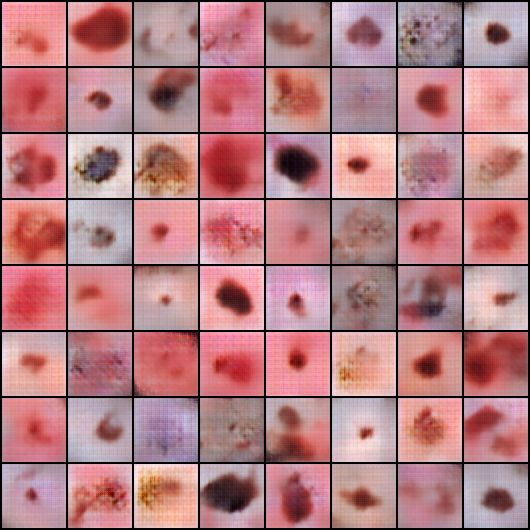
\includegraphics[width=5in]{images/fake_samples_epoch_109.png}
    \caption{First prototype output after 109 epochs}
    \label{fig:prototype-output}
\end{figure}

\begin{lstlisting}
import torch.nn as nn


class Discriminator(nn.Module):
    def __init__(self, image_channels, features_d, ngpu=1):
        super().__init__()
        self.ngpu = ngpu
        self.disc = nn.Sequential(
            # input dims: N x 3 x 64 x 64
            nn.Conv2d(
                image_channels, features_d, kernel_size=4, stride=2, padding=1
            ),
            nn.LeakyReLU(0.2),
            # _block(in_channels, out_channels, kernel_size, stride, padding)
            self._block(features_d, features_d * 2, 4, 2, 1),
            self._block(features_d * 2, features_d * 4, 4, 2, 1),
            self._block(features_d * 4, features_d * 8, 4, 2, 1),
            # Conv2d down to 1x1
            nn.Conv2d(features_d * 8, 1, kernel_size=4, stride=2, padding=0),
            nn.Sigmoid(),
        )

    def _block(self, in_channels, out_channels, kernel_size, stride, padding):
        return nn.Sequential(
            nn.Conv2d(
                in_channels,
                out_channels,
                kernel_size,
                stride,
                padding,
                bias=False,
            ),
            nn.BatchNorm2d(out_channels),
            nn.LeakyReLU(0.2),
        )

    def forward(self, x):
        if x.is_cuda and self.ngpu > 1:
            output = nn.parallel.data_parallel(self.disc, x, range(self.ngpu))
        else:
            output = self.disc(x)
        return output.view(-1, 1).squeeze(1)


class Generator(nn.Module):
    def __init__(self, noise_vector, image_channels, features_g, ngpu=1):
        super().__init__()
        self.ngpu = ngpu
        self.gan = nn.Sequential(
            # input dims: N x noise_vector x 1 x 1
            self._block(noise_vector, features_g * 16, 4, 1, 0),  # img: 4x4
            self._block(features_g * 16, features_g * 8, 4, 2, 1),  # img: 8x8
            self._block(features_g * 8, features_g * 4, 4, 2, 1),  # img: 16x16
            self._block(features_g * 4, features_g * 2, 4, 2, 1),  # img: 32x32
            nn.ConvTranspose2d(
                features_g * 2, image_channels, kernel_size=4, stride=2, padding=1
            ),
            # output dims: N x 3 x 64 x 64
            nn.Tanh(),
        )

    def _block(self, in_channels, out_channels, kernel_size, stride, padding):
        return nn.Sequential(
            nn.ConvTranspose2d(
                in_channels,
                out_channels,
                kernel_size,
                stride,
                padding,
                bias=False,
            ),
            nn.BatchNorm2d(out_channels),
            nn.ReLU(),
        )

    def forward(self, x):
        if x.is_cuda and self.ngpu > 1:
            output = nn.parallel.data_parallel(self.gan, x, range(self.ngpu))
        else:
            output = self.gan(x)
        return output


def init_weights(model):
    """
    Initialize weights based on DC-GAN paper
    :param model:
    """
    for m in model.modules():
        if isinstance(m, (nn.Conv2d, nn.ConvTranspose2d, nn.BatchNorm2d)):
            nn.init.normal_(m.weight.data, 0.0, 0.02)
\end{lstlisting}

\newpage
\chapter{Week 04: Implementation 3}
\section{Extensions to prototype, debugging.}
\paragraph{
 This week we have tried two different ideas: One was to fine-tune the existing prototype to return better results than last time and the other idea was to create a W-GAN. \\
 For the first we adjusted the learning rate several times and tried to run the learning longer, so more than 109 epochs. We also tried to change the batch sizes to 16, 32, and 64. These measures sadly did not yield significantly better results. Next on the list is to try to train on the full resolution of the dataset instead of just using the lowered resolution and cropped dataset. Also we want to test out different input noise vector sizes.\\ 
 For the second idea, we tried the W-GAN, which was already implemented from one of our members for a past project. That implementation worked in MNIST, but applied to our dataset, it did not perform. Currently we are trying out different hyperparameters and are trying to figure out the reason for the W-GAN not performing. Another idea was to try the W-GAN with gradient penalty. Hopefully we have better results to report for next week.
}
